\chapter{Fundamentação Teórica}
\label{chap:fundament}

\section{Métodos de posicionamento GNSS}
\noindent

De acordo com \cite{monico2008}, posicionamento diz respeito à determinação da posição de objetos com relação a um determinado referencial. Neste contexto, o posicionamento pode ser dividido em: \textit{Absoluto} e \textit{Relativo}. Absoluto, quando as coordenadas estão diretamente associadas ao geocentro; e Relativo, quando são determinadas em relação a um referencial materializado por um ou mais vértices com coordenadas conhecidas. Outra classificação que pode ser feita é quanto ao movimento do objeto a ser posicionado em relação ao referencial. Pode-se dividir em \textit{cinemático}, quando o objeto está em movimento em relação ao referencial ou \textit{estático} quando esse está em repouso.

Ainda não existe uma terminologia padrão para os métodos de posicionamento GNSS junto a comunidade científica, desta forma, neste PFC será adotada a classificação de \cite{monico2008}:
\begin{itemize}
    \item Posicionamento absoluto;
    \item Posicionamento relativo;
    \item Posicionamento com DGPS.
\end{itemize}

Serão aplicados no presente trabalho os métodos de RTPPP e PPP-RTK que enquadram-se em posicionamento absoluto e o método de RTK que é classificado como posicionamento relativo.

\section{Protocolo de transmissão de dados GNSS}
\noindent

Para realizar os métodos de posicionamento GNSS por vezes são necessários protocolos de transmissão que possibilitem a correta comunicação entre as peças envolvidas no método; o RTCM é um padrão empregado em operações com GPS envolvendo posicionamento nos modos DGPS e RTK.

O padrão RTCM foi desenvolvido pela \textit{Radio Technical Commission for Maritime Services}. Este padrão de formato de dados é utilizado para a transmissão de informações entre uma estação de referência e outra remota, geralmente em movimento, possibilitando posicionamento em tempo real.

Na área de navegação e posicionamento, o padrão mais comum é aquele conhecido como padrão SC-104 (geralmente chamado apenas de padrão RTCM). Em meados da década de 80, a RTCM estabeleceu um comitê especial, de número 104. O objetivo inicial deste comitê especial era o de projetar um formato padrão que permitisse a transmissão de informações, das mais diversas, relacionadas com o emprego da tecnologia GPS. Este objetivo se expandiu e atualmente o formato possibilita a transmissão de informações para outros sistemas GNSS (tais com o GLONASS) \citep{Navipedia2019}.


\section{Posicionamento Por Ponto Preciso (PPP)}
\noindent

Com o intuito de entender melhor a base para os métodos de RTPPP e PPP-RTK, será tratado a respeito do método PPP. O método do PPP se utiliza  de efemérides precisas e correções de relógios dos satélites. Tal termo foi utilizado primeiramente por \cite{heroux1995gps}. Essa metodologia de posicionamento se utiliza, assim como as outras, de três componentes: as observações; os modelos de correção; e o processo de ajustamento \citep{cunha2016_PPP}. O seu ganho de precisão em relação ao \textit{Posicionamento por Ponto Absoluto} é a utilização de observações e métodos para correção das observações. As observações utilizadas englobam as efemérides e correções dos relógios dos satélites. A utilização dessas observações combinada ao modelos de correção e ajustamento proporciona ao PPP uma precisão centimétrica. O PPP divide-se em duas fases:

\begin{enumerate}
    \item Centrais de análise recebe os dados de controle de GNSS e cria produtos precisos;
    \item Os produtos de elevada precisão são utilizados para processar os dados coletados pelo receptor GNSS.
\end{enumerate}

É importante salientar que para a realização do PPP é necessário um receptor GNSS de dupla frequência. \cite{cunha2016_PPP} cita \cite{kouba2001precise} ao caracterizar o modelo tradicional de PPP:
\begin{itemize}
    \item Combinação de observações de dupla frequência da pseudodistância e da fase da portadora para criar uma observação \textit{ion-free} (IF);
    \item Implementação de um filtro sequencial para o procedimento de ajuste;
    \item Determinação do atraso troposférico zenital húmido como uma incógnita adicional;
    \item Utilização de modelos para estimar o valor das restantes fontes de erro.
\end{itemize}


\subsection{Modelo matemático do PPP}
\noindent

A seguir será apresentado o modelo funcional do PPP. Utilizando dados de um receptor GNSS de dupla frequência, as equações de pseudodistância e fase da onda portadora parametrizada com a aplicação da combinação ion-free (IF) podem ser escritas da seguinte forma \citep{marques2012ppp}:

\begin{equation}
    \label{eq:PD}
    PD_{IF_r}^{s}=\rho_r^s+c.(dt_r(t_r)+dt^s(t^t))+m_f.Zwd+\varepsilon_{PD_r^{s}}
\end{equation}

\begin{equation}
    \label{eq:lambda}
    \lambda_{IF}.\phi_{IF_r}^{s}=\rho_r^s+c.(dt_r(t_r)-dt^s(t^t))+\lambda_{IF}.N_{IF}+m_f.Zwd+\varepsilon_{\phi_r^{s}}
\end{equation}

Nas equações \ref{eq:PD} e \ref{eq:lambda} tem-se que:
\begin{itemize}
    \item $PD_{IF_r}^{s}$ - pseudodistância da \textit{ion-free} (metros);
    \item $\lambda_{IF}.\phi_{IF_r}^{s}$ - fase da \textit{ion-free} (metros);
    \item $\rho_r^s$ - distância geométrica entre receptor r e o satélite s;
    \item $dt_r(t_r)$ - erro do relógio do receptor no instante de recepção $t_r$;
    \item $dt^s(t^t)$ - erro do relógio do receptor no instante de recepção $t^t$
    \item $N_{IF}$ - ambiguidade da \textit{ion-free};
    \item Zwd - atraso troposférico úmido na direção do zênite;
    \item $m_f$ - função de mapeamento do Zwd para a direção receptor-satélite; e
    \item $\varepsilon_{PD_r^{s}}$ e $\varepsilon_{\phi_r^{s}}$ - os erros aleatórios e não modelados nas equações \textit{ion-free} de pseudodistância e fase.
\end{itemize}

As equações \ref{eq:PD} e \ref{eq:lambda} apresentam modelos não lineares e a equação linearizada considerando um receptor \textit{r} e o satélite $s_i$, pode ser escrita como \citep{marques2014ppp}:
\begin{equation}
\label{lin_ppp}
E
\begin{Bmatrix}
\begin{bmatrix}
\Delta PD_{IF_r}^{s_i}\\
\Delta \lambda_{IF}.\phi_{IF_r}^{s_i}
\end{bmatrix}
\end{Bmatrix}
=AX=
\begin{bmatrix}
-\frac{X^{s_i}-X^0_r}{(\rho^{s_i}_r)^0} & -\frac{Y^{s_i}-Y^0_r}{(\rho^{s_i}_r)^0}& -\frac{Z^{s_i}-Z^0_r}{(\rho^{s_i}_r)^0} & 1 & M_f & 0\\
-\frac{X^{s_i}-X^0_r}{(\rho^{s_i}_r)^0} & -\frac{Y^{s_i}-Y^0_r}{(\rho^{s_i}_r)^0}& -\frac{Z^{s_i}-Z^0_r}{(\rho^{s_i}_r)^0} & 1 & M_f & \lambda_{IF}
\end{bmatrix}
\begin{bmatrix}
\Delta X_r\\
\Delta Y_r\\
\Delta Z_r\\
\Delta c.dt_r\\
Z_{wd}\\
N^{s_i}_{IF}
\end{bmatrix}
\end{equation}

Na equação \ref{lin_ppp}:
\begin{itemize}
    \item $\Delta PD_{IF_r}^{s_i}$ - diferença entre a pseudodistância observada e a calculada (vetor L para pseudodistância);
    \item $\Delta \lambda_{IF}.\phi_{IF_r}^{s_i}$ - diferença entre a fase observada e a calculada (vetor L para fase);
    \item $(\rho^{s_i}_r)^0$ - distância geométrica calculada em função dos parâmetros aproximados; e
    \item E\{.\} - representa o operador de esperança matemática.
    \item Os termos $\Delta X_r$, $\Delta Y_r$, $\Delta Z_r$, $dt_r$, $Z_{wd}$ e $N_{IF}$ são as correções aos parâmetros incógnitos, ou seja, as coordenadas da estação, erro do relógio do receptor, troposfera e ambiguidade.
\end{itemize}


\section{Posicionamento Por Ponto Preciso em tempo real (RTPPP)}

\begin{figure}[H]
\centering
% ---
% Taken from https://cremeronline.com/LaTeX/minimaltikz.pdf
\tikzstyle{block} = [rectangle, draw, fill=white, text width=6em, text centered, rounded corners, node distance=2cm, minimum height=2em]
\tikzstyle{cloud} = [draw, ellipse,fill=white, node distance=2cm, minimum height=2em]
\fbox{
\begin{tikzpicture}
%\node[inner sep=0pt] (sat) at (0,0) {
\includegraphics[width=.15\textwidth]{satelite.png}};
    
\node[inner sep=0pt] (rec1) at (0,-10) [label=below:Receptor 1] {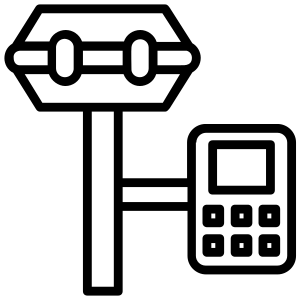
\includegraphics[width=.05\textwidth]{receiver.png}};
\node[inner sep=0pt] (rec2) at (2.5,-10) [label=below:Receptor 2] {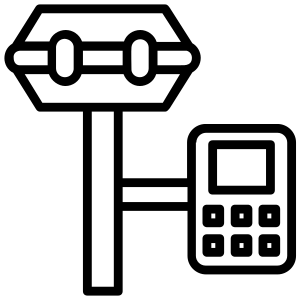
\includegraphics[width=.05\textwidth]{receiver.png}};
\node (recponto) at (5,-10) {...};
\node[inner sep=0pt] (recn) at (7.5,-10) [label=below:Receptor n] {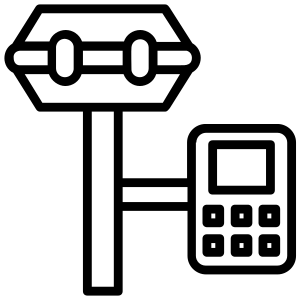
\includegraphics[width=.05\textwidth]{receiver.png}};


\node[inner sep=0pt] (laptop) at (5,-5) [label=left:Software BNC] {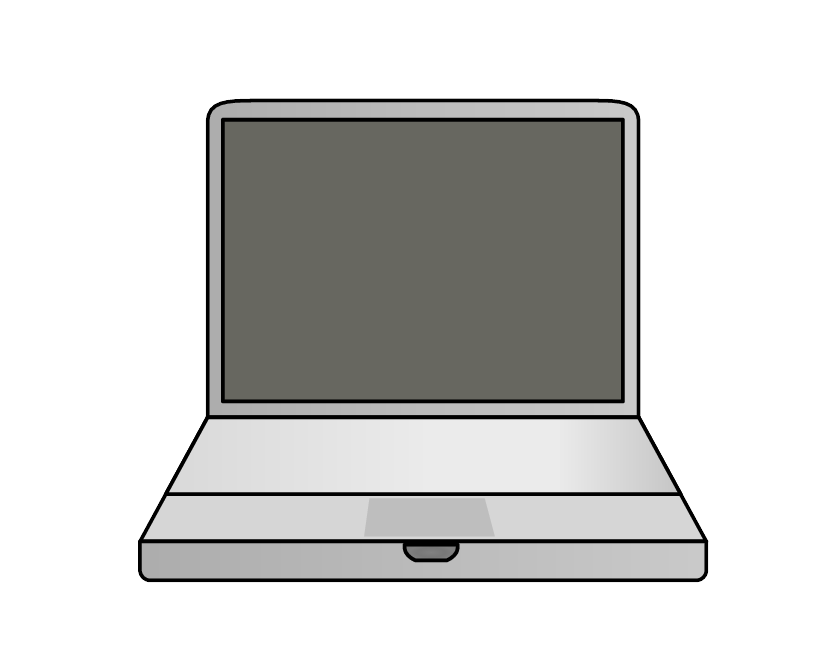
\includegraphics[width=.10\textwidth]{laptop.png}};

\node [block] (caster1) at (3,-8) {Caster 1};

\node[cloud] (ppp) at (2,0) {PPP em Tempo Real};
 
%\node [block] (relogio) at (10,-8) {Software Solução Relógios};

\node [block] (caster2) at (12,-2) {Caster 2};
\node[inner sep=0pt] (rec) at (10,-5.5) [label=below:Receptor Usuário] {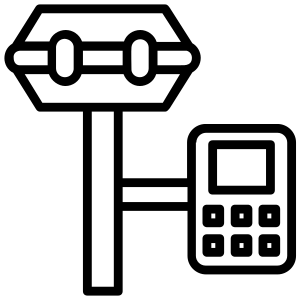
\includegraphics[width=.065\textwidth]{receiver.png}};



\draw[->,thick,shorten >=5pt] (rec1.north) -- (caster1);
\draw[->,thick,shorten >=3pt] (rec2.north) -- (caster1);
\draw[->,thick,shorten >=3pt] (recponto.north) -- (caster1);
\draw[->,thick,shorten >=5pt] (recn.north) -- (caster1);

\draw[->,thick] (caster1) -- (laptop)
    node[midway,fill=white] {Dados GNSS e Órbitas transmitidas};
    
%\draw[->,thick] (relogio) -- (laptop)    node[midway,fill=white] {Envio ao usuário};
    
\draw[->,thick] (caster2) -- (laptop) node[midway,fill=white] {Correção Órbitas/Relógios};
\draw[->,thick] (rec) -- (laptop) node[midway,fill=white] {Porta Serial};

\draw[<->,thick,shorten >=3pt] (laptop) -- (ppp) node[midway,fill=white] {Solução \textit{float} ambiguidades};;

\end{tikzpicture}}
% ---
\caption{Esquema RTPPP.}
\end{figure}


\noindent

O RTPPP se utiliza do mesmo método do PPP entretanto requer a disponibilidade em tempo real das órbitas precisas e das correções ou erros dos relógios dos satélites (não sincronização do relógio do satélite com o sistema de tempo GNSS) \citep{marques2012ppp}. Essa necessidade é devido ao fato do RTPPP proporcionar o posicionamento em tempo real. 

O RTPPP se utiliza da solução de ambiguidades pelo método ''\textit{float}'' e pode ser realizado com um receptor GNSS de dupla frequência conectado via porta serial com um computador. Esse computador deve possuir acesso a internet pois receberá dados de dois \textit{Caster}. O \textit{Caster} 1 envia para o usuário dados GNSS de outros receptores além das órbitas transmitidas dos satélites. O \textit{Caster} 2 envia ao usuário as informações de órbita e relógio do satélite. Nessas informações estão contidas a solução dos relógios dos satélites que atenua os erros dos relógios dos satélites. É possível então, em posse dos dados recebidos pelos \textit{Caster} 1 e 2 e das observáveis GNSS obtidas no receptor GNSS em questão, processar os dados e realizar o PPP em tempo real.



\newpage
\section{Introdução ao método PPP-RTK}
\noindent

O método PPP-RTK é um complemento ao PPP onde a precisão e acurácia são melhores. De acordo com \cite{wubbena2005ppp}, as limitações do método PPP podem ser superadas utilizando uma rede RTK, como as redes RTK podem obter todos os erros GNNS em tempo real o usuário pode resolver as ambiguidades e obter um nível de acurácia superior ao método PPP.

O conceito de PPP aliado a solução de ambiguidades é a síntese do PPP-RTK. A seguir encontra-se uma tabela que explicita as diferenças entre o PPP e o PPP-RTK:

\begin{table}[H]
\begin{center}
\begin{tabular}{c|c|c|}
\cline{2-3}
                                                      & \textbf{\textit{PPP}}            & \textbf{\textit{PPP-RTK}}                 \\ \hline
\multicolumn{1}{|c|}{\textbf{Tamanho da rede}}        & global                  & local/regional/	global           \\ \hline
                                                      & \multicolumn{2}{c|}{\textit{Primary state information}}    \\ \hline
\multicolumn{1}{|c|}{\textbf{Órbitas dos satélites}}  & fornecido               & fornecido                        \\ \hline
\multicolumn{1}{|c|}{\textbf{Relógios dos satélites}} & fornecido               & fornecido                        \\ \hline
\multicolumn{1}{|c|}{\textbf{Ionosfera}}              & corrigido               & fornecido                        \\ \hline
\multicolumn{1}{|c|}{\textbf{Troposfera}}             & estimado                & fornecido                        \\ \hline
\multicolumn{1}{|c|}{\textbf{Relógio do receptor}}    & estimado                & estimado                         \\ \hline
                                                      & \multicolumn{2}{c|}{\textit{Ambiguidade da fase e sinal}} \\ \hline
\multicolumn{1}{|c|}{\textbf{L1/ L2 / L0}}            & -/ - / +                & +/ + / +                         \\ \hline
\multicolumn{1}{|c|}{\textbf{Tempo de integração}}    & 30... 1800 s            & 10... 50 s                       \\ \hline
                                                      & \multicolumn{2}{c|}{\textit{Acurácia}}                     \\ \hline
\multicolumn{1}{|c|}{\textbf{3D estático}}            & $\sim$5 cm              & 1... 3 cm                        \\ \hline
\multicolumn{1}{|c|}{\textbf{RTK 3D}}                 & 15... 20 cm             & 1... 3 cm                        \\ \hline
\end{tabular}
\end{center}
\caption{Diferenças entre PPP e PPP-RTK. Adaptado de \cite{wubbena2005ppp}.}
\label{tableref}
\end{table}

Conceitualmente, o PPP-RTK é bastante similar ao método RTPPP, com a diferença que se utiliza de uma solução de ambiguidades \textit{fixa} o invés de \textit{float}. Nesse método portando o \textit{Caster} 2 proporciona uma solução de ambiguidades do tipo \textit{fixa}, mais precisa que a solução \textit{float}. A seguir um esquema que explicita o método PPP-RTK:


\begin{figure}[H]
\centering
% ---
% Taken from https://cremeronline.com/LaTeX/minimaltikz.pdf
\tikzstyle{block} = [rectangle, draw, fill=white, text width=6em, text centered, rounded corners, node distance=2cm, minimum height=2em]
\tikzstyle{cloud} = [draw, ellipse,fill=white, node distance=2cm, minimum height=2em]
\fbox{
\begin{tikzpicture}
%\node[inner sep=0pt] (sat) at (0,0) {
\includegraphics[width=.15\textwidth]{satelite.png}};
    
\node[inner sep=0pt] (rec1) at (0,-10) [label=below:Receptor 1] {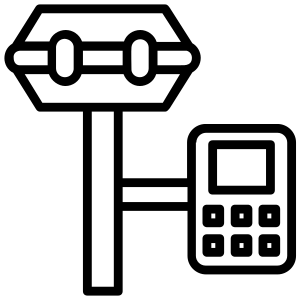
\includegraphics[width=.05\textwidth]{receiver.png}};
\node[inner sep=0pt] (rec2) at (2.5,-10) [label=below:Receptor 2] {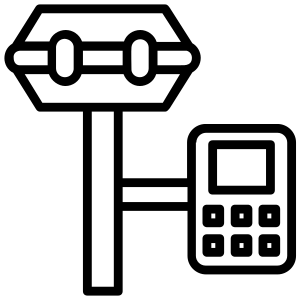
\includegraphics[width=.05\textwidth]{receiver.png}};
\node (recponto) at (5,-10) {...};
\node[inner sep=0pt] (recn) at (7.5,-10) [label=below:Receptor n] {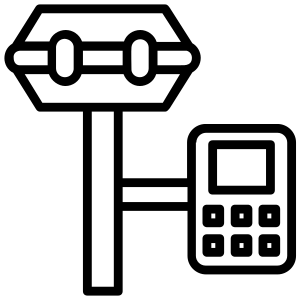
\includegraphics[width=.05\textwidth]{receiver.png}};


\node[inner sep=0pt] (laptop) at (5,-5) [label=left:Software BNC] {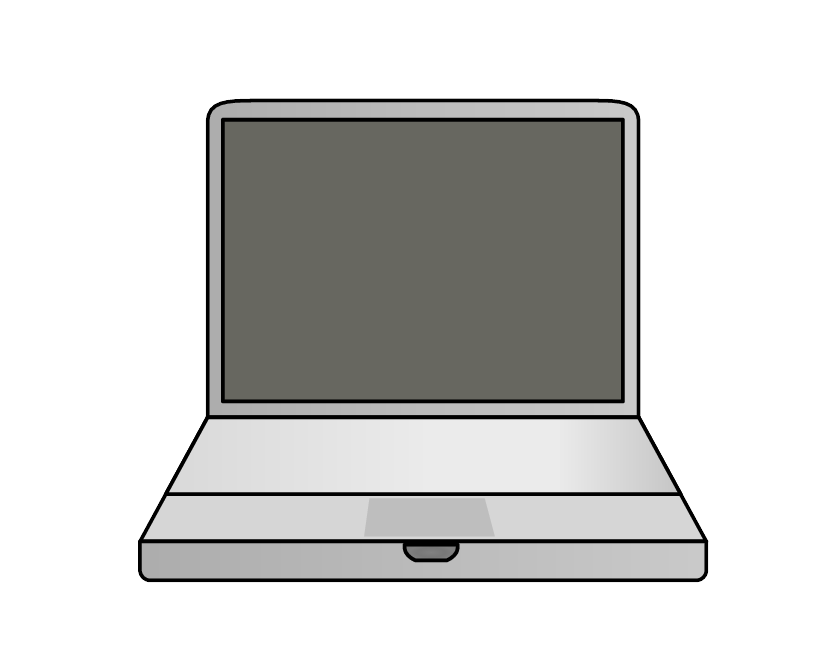
\includegraphics[width=.10\textwidth]{laptop.png}};

\node [block] (caster1) at (3,-8) {Caster 1};

\node[cloud] (ppp) at (2,0) {PPP em Tempo Real};
 
%\node [block] (relogio) at (10,-8) {Software Solução Relógios};

\node [block] (caster2) at (12,-2) {Caster 2};
\node[inner sep=0pt] (rec) at (10,-6) [label=below:Receptor Usuário] {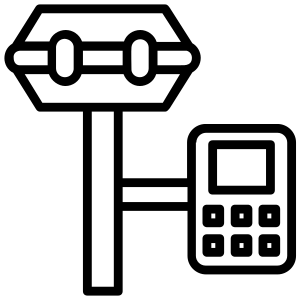
\includegraphics[width=.065\textwidth]{receiver.png}};



\draw[->,thick,shorten >=5pt] (rec1.north) -- (caster1);
\draw[->,thick,shorten >=3pt] (rec2.north) -- (caster1);
\draw[->,thick,shorten >=3pt] (recponto.north) -- (caster1);
\draw[->,thick,shorten >=5pt] (recn.north) -- (caster1);

\draw[->,thick] (caster1) -- (laptop)
    node[midway,fill=white] {Dados GNSS e Órbitas transmitidas};
    
%\draw[->,thick] (relogio) -- (laptop)    node[midway,fill=white] {Envio ao usuário};
    
\draw[->,thick] (caster2) -- (laptop) node[midway,fill=white] {Correção Órbitas/Relógios};
\draw[->,thick] (rec) -- (laptop) node[midway,fill=white] {Porta Serial};

\draw[<->,thick,shorten >=3pt] (laptop) -- (ppp) node[midway,fill=white] {Solução \textit{fixa} ambiguidades};;

\end{tikzpicture}}
% ---
\caption{Esquema PPP-RTK.}
\end{figure}


\section{RTK utilizando protocolo NTRIP}
\noindent

O georreferenciamento de áreas no Brasil é um campo de extrema importância e o desenvolvimento de novas tecnologias apoiadas na rede de telefonia móvel vem sendo aprimorado. Nesse contexto, destaca-se o uso da tecnologia RTK NTRIP, que utiliza a rede de telefonia móvel para receber correções em tempo real, através da internet \citep{LENZ2004}.

O método RTK NTRIP - \textit{Networked Transport of RTCM} via \textit{Internet Protocol} - possibilita o usuário, por meio da internet, receber as correções das estações RBMC.

De acordo com \cite{LENZ2004} , esse método foi desenvolvido pela Agência Federal de Cartografia e Geodésia da Alemanha, juntamente com a Universidade de Dortmund e a Trimble. O principal objetivo foi utilizar a internet como uma alternativa às tecnologias existentes de correção via rádio e telefonia celular.

O sistema é composto de receptores que enviam continuamente dados no formato RCTM a um servidor denominado \textit{''Caster''} e um aplicativo denominado ''Cliente'' localizado no equipamento do interessado a receber as correções. Suas principais características são:

\begin{itemize}
    \item baseado em HTTP (Hipertext Transfer Protocol);
    \item disponibilidade de distribuir qualquer tipo de dados GNSS em fluxo;
    \item capacidade de aceitar uma grande quantidade de usuários simultaneamente;
    \item o acesso aos dados é realizado de forma segura sem a necessidade de o usuário estar em contato direto com as estações de referência;
    \item habilitado a fornecer o fluxo de dados através de qualquer rede móvel TCP/IP (\textit{Transfer Control Protocol / Internet Protocol});
    \item a largura de banda necessária para disseminar as correções GNSS é relativamente pequena. Aproximadamente 5Kb/s para RTK.
\end{itemize}


O NTRIP é basicamente composto por três componentes; o NTRIP \textit{Server}, o NTRIP \textit{Caster} e o NTRIP \textit{Client}.



\begin{figure}[!htb]
\centering
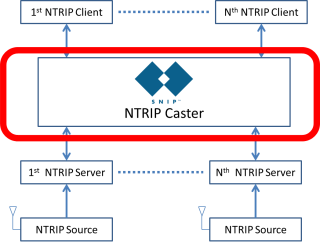
\includegraphics[scale=2.0]{img/nnnnnnn.png} %scale eh o tamanho que a figura vai ficar
\caption{Sitema NTRIP. \citep{snip}}
\label{Rotulo}
\end{figure}


O referido método é mais operacional em relação ao RTPPP e PPP-RTK pois não necessita de um computador conectador ao receptor GNSS. O receptor conectado a internet (via chip GSM) recebe informações do \textit{Caster} 1 (que faz o papel de estação base) e do \textit{Caster} 2 (que fornece informações de órbita e relógio dos satélites).

Sua vantagem em relação ao RTK convencional é ausência do link de rádio. O link de rádio que conecta a estação base a estação \textit{rover} pode ser prejudicado por obstáculos entre as estações. Contudo, pode-se ter problemas na solução de ambiguidades se a estação base conectada à internet estiver muito distante. No RTK/NTRIP o \textit{Caster} 1 faz o papel de estação base e essas informações chegam via internet. A seguir um esquema que exemplifica o RTK/NTRIP:

\begin{figure}[H]
\centering
% ---
% Taken from https://cremeronline.com/LaTeX/minimaltikz.pdf
\tikzstyle{block} = [rectangle, draw, fill=white, text width=6em, text centered, rounded corners, node distance=2cm, minimum height=2em]
\tikzstyle{cloud} = [draw, ellipse,fill=white, node distance=2cm, minimum height=2em]
\fbox{
\begin{tikzpicture}
%\node[inner sep=0pt] (sat) at (0,0) {
\includegraphics[width=.15\textwidth]{satelite.png}};
    
\node[inner sep=0pt] (rec1) at (0,-10) [label=below:Receptor 1] {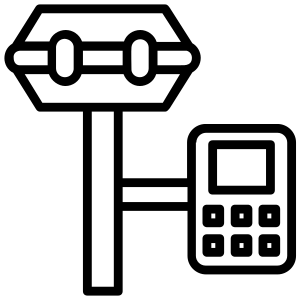
\includegraphics[width=.05\textwidth]{receiver.png}};
\node[inner sep=0pt] (rec2) at (2.5,-10) [label=below:Receptor 2] {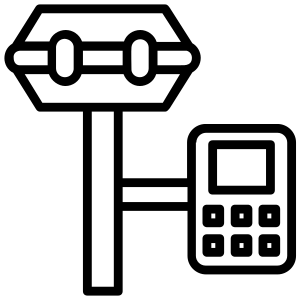
\includegraphics[width=.05\textwidth]{receiver.png}};
\node (recponto) at (5,-10) {...};
\node[inner sep=0pt] (recn) at (7.5,-10) [label=below:Receptor n] {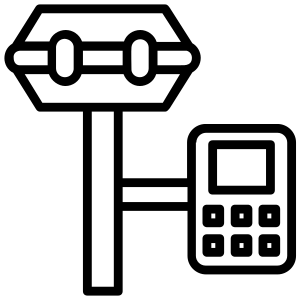
\includegraphics[width=.05\textwidth]{receiver.png}};


\node[inner sep=0pt] (laptop) at (7,-5) [label=right:Receptor usuário] {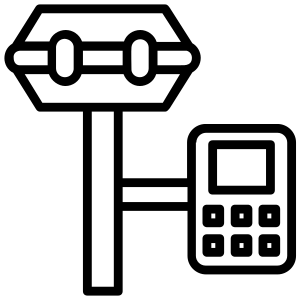
\includegraphics[width=.10\textwidth]{receiver.png}};

\node [block] (caster1) at (3,-8) {Caster 1};

\node[cloud] (ppp) at (2,-2) {RTK/NTRIP};
 
%\node [block] (relogio) at (10,-8) {Software Solução Relógios};

%\node [block] (caster2) at (12,0) {Caster 2};




\draw[->,thick,shorten >=5pt] (rec1.north) -- (caster1);
\draw[->,thick,shorten >=3pt] (rec2.north) -- (caster1);
\draw[->,thick,shorten >=3pt] (recponto.north) -- (caster1);
\draw[->,thick,shorten >=5pt] (recn.north) -- (caster1);

\draw[->,thick] (caster1) -- (laptop)
    node[midway,fill=white] {Comunicação NTRIP};
    
%\draw[->,thick] (relogio) -- (laptop)    node[midway,fill=white] {Envio ao usuário};
    
%\draw[->,thick] (caster2) -- (laptop);% node[midway,fill=white] {Solução \textit{fixa} ambiguidades};


\draw[<->,thick,shorten >=3pt] (laptop) -- (ppp) {};

\end{tikzpicture}}
% ---
\caption{Esquema RTK/NTRIP.}
\end{figure}

\section{Sistema Geodésico Local}
O Sistema Geodésico Local (SGL) é um sistema que é composto por três eixos (e,n,u) que são mutuamente ortogonais. O eixo ''n'' aponta em direção ao norte geodésico, o eixo ''e'' aponta para a direção leste, sendo que os eixos ''n'' e ''e'' estão contidos no plano topocêntrico. Por fim, o eixo ''u'' coincide com a normal do elipsoide que passa pelo vértice escolhido como a origem do sistema \citep{INCRA}. A figura a seguir ilustra o SGL.

\begin{figure}[H]
\centering
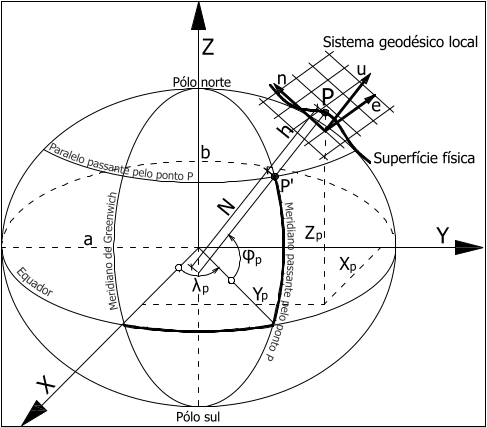
\includegraphics[scale=0.7]{img/sgl.png} %scale eh o tamanho que a figura vai ficar
\caption{Sitema Geodésico Local. \citep{ibge_imoveis}}
\label{Rotulo}
\end{figure}

O seguinte modelo matemático é utilizado para calcular as coordenadas geodésicas locais:

\small
\begin{equation}
\label{sgl_mod_mat}
\begin{bmatrix}
e\\
n\\
u
\end{bmatrix}
=
\begin{bmatrix}
1 & 0 & 0\\
0 & \sin{\varphi_0} & \cos{\varphi_0}\\
0 & -\cos{\varphi_0} & \sin{\varphi_0}
\end{bmatrix}
\begin{bmatrix}
-\sin{\lambda_0} & \cos{\lambda_0}\\
-\cos{\lambda_0} & -\sin{\lambda_0} & 0\\
0 & 0 & 1
\end{bmatrix}
\begin{bmatrix}
X-X_0\\
Y-Y_0\\
Z-Z_0
\end{bmatrix}
\end{equation}
\normalsize

Em que:
\begin{itemize}
    \item \textit{e, n, u} - são as coordenadas cartesianas locais do vértice de interesse;
    \item \textit{X, Y, Z} - são as coordenadas cartesianas geocêntricas do vértice de interesse;
    \item $\varphi_0$, $\lambda_0$ - são a latitude e a longitude adotadas como origem do sistema;
    \item $X_0$, $Y_0$, $Z_0$ - são as coordenadas cartesianas geocêntricas adotadas como origem do sistema.
\end{itemize}